%%%%%%%%%%%%%%%%%%%%%%%%%%%%%%%%%%%%%%%%%%%%%%%%%%%%%%%%%%
%%% Document
%%%%%%%%%%%%%%%%%%%%%%%%%%%%%%%%%%%%%%%%%%%%%%%%%%%%%%%%%%
\documentclass[pdftex, a4paper,11pt, twoside, ngerman]{report}
% \documentclass[11pt,xcolor=dvipsnames]{beamer}

% \usepackage[utf8x]{inputenc} 		%für deutsche zeichen äüö ohne kile auto-ersetzen
% \usepackage[ansinew]{inputenc}	%kile auto-ersetzen: einstellungen->latex:general-> hacken bei special characters
% \usepackage[UKenglish]{babel}  	%Englisch
\usepackage[ngerman]{babel}  	%Deutsch



%%%%%%%%%%%%%%%%%%%%%%%%%%%%%
%%% Geometry
%%%%%%%%%%%%%%%%%%%%%%%%%%%%%
% \usepackage{showframe}
\usepackage[scale=0.8, hmarginratio=4:2]{geometry}
  \geometry{textheight=1.05\textheight, textwidth=.95\textwidth, marginparwidth=25 pt}



%%%%%%%%%%%%%%%%%%%%%%%%%%%%%
%%% Packages (aus header datei)
%%%%%%%%%%%%%%%%%%%%%%%%%%%%%
\IfFileExists{header_TobiasBrauell-DOCUMENT.tex}{% Copyright © 2014 Tobias Brauell <tobiasbrauell@gmail.com>

% This is my general purpose LaTeX header file for writing German documents.
% Ideally, you include this using a simple ``\input{header.tex}`` in your main
% document and start with ``\title`` and ``\begin{document}`` afterwards.

% If you need to add additional packages, I recommend not doing this in this
% file, but in your main document. That way, you can just drop in a new
% ``header.tex`` and get all the new commands without having to merge manually.

%%%%%%%%%%%%%%%%%%%%%%%%%%%%%
%%% Locale, date
%%%%%%%%%%%%%%%%%%%%%%%%%%%%%
\usepackage[UKenglish]{isodate}



%%%%%%%%%%%%%%%%%%%%%%%%%%%%%
%%% Margins and other spacing
%%%%%%%%%%%%%%%%%%%%%%%%%%%%%
\usepackage[activate]{pdfcprot}
% \usepackage[parfill]{parskip}
\usepackage{setspace}
  \setlength{\columnsep}{2 cm}
  \setlength{\parindent}{0 pt}


%%%%%%%%%%%%%%%%%%%%%%%%%%%%%
%%% Input encoding
%%%%%%%%%%%%%%%%%%%%%%%%%%%%%
\usepackage[T1]{fontenc}
\usepackage[utf8x]{inputenc}



%%%%%%%%%%%%%%%%%%%%%%%%%%%%%
%%% Indexing
%%%%%%%%%%%%%%%%%%%%%%%%%%%%%
\usepackage{makeidx}
  \makeindex



%%%%%%%%%%%%%%%%%%%%%%%%%%%%%
%%% Blindtext
%%%%%%%%%%%%%%%%%%%%%%%%%%%%%
\usepackage{blindtext}


%%%%%%%%%%%%%%%%%%%%%%%%%%%%%
%%% Global Counter
%%%%%%%%%%%%%%%%%%%%%%%%%%%%%



%%%%%%%%%%%%%%%%%%%%%%%%%%%%%
%%% Geometry
%%%%%%%%%%%%%%%%%%%%%%%%%%%%%
\usepackage{layout}
% \usepackage[scale=0.8]{geometry}
%   \geometry{textheight=1.05\textheight, marginparwidth=50 pt}

% \usepackage{multirow}
% \usepackage{dcolumn}



%%%%%%%%%%%%%%%%%%%%%%%%%%%%%
%%% Pagestyle
%%%%%%%%%%%%%%%%%%%%%%%%%%%%%
% \usepackage{fancyhdr}
% \usepackage{microtype} 

% \pagestyle{fancy}



%%%%%%%%%%%%%%%%%%%%%%%%%%%%%
%%% Fonts/Colors
%%%%%%%%%%%%%%%%%%%%%%%%%%%%%
\usepackage{lmodern}
\usepackage{xcolor}
% This replaces all fonts with Bitstream Charter, Bitstream Vera Sans and
% Bitstream Vera Mono. Math will be rendered in Charter.
% \usepackage[charter, greekuppercase=italicized]{mathdesign}
% \usepackage{beramono}
% \usepackage{berasans}

% Bold, sans-serif tensors. This fragment is taken from “egreg” from
% http://tex.stackexchange.com/a/82747/8945 and licensed under `CC-BY-SA
% <https://creativecommons.org/licenses/by-sa/3.0/>`_.
% \usepackage{bm}
%   \DeclareMathAlphabet{\mathsfit}{\encodingdefault}{\sfdefault}{m}{sl}
%   \SetMathAlphabet{\mathsfit}{bold}{\encodingdefault}{\sfdefault}{bx}{sl}
%   \newcommand{\tens}[1]{\bm{\mathsfit{#1}}}

% Bold vectors.
% \renewcommand{\vec}[1]{\boldsymbol{#1}}



%%%%%%%%%%%%%%%%%%%%%%%%%%%%%
%%% Code/Listings
%%%%%%%%%%%%%%%%%%%%%%%%%%%%%
\usepackage{listings}



%%%%%%%%%%%%%%%%%%%%%%%%%%%%%
%%% Enumerations
%%%%%%%%%%%%%%%%%%%%%%%%%%%%%
\usepackage{enumitem}
% \usepackage{paralist}


%%%%%%%%%%%%%%%%%%%%%%%%%%%%%
%%% Figures
%%%%%%%%%%%%%%%%%%%%%%%%%%%%%
% \usepackage[pdftex]{graphicx}
\usepackage{graphicx}
\usepackage{epsfig}
\usepackage{epstopdf}
\usepackage{subfigure}
\usepackage{wrapfig}
\makeatletter \newcommand\hyper@makecurrent[1]{} \makeatother
\usepackage{caption}
% \usepackage{subcaption}

\addto\captionsUKenglish{\renewcommand{\figurename}{Fig.}}
\addto\captionsngerman{\renewcommand{\figurename}{Abb.}}



%%%%%%%%%%%%%%%%%%%%%%%%%%%%%
%%% PDF Pages
%%%%%%%%%%%%%%%%%%%%%%%%%%%%%
\usepackage{pdfpages}



%%%%%%%%%%%%%%%%%%%%%%%%%%%%%
%%% Personal Graphics
%%%%%%%%%%%%%%%%%%%%%%%%%%%%%
\usepackage{tikz}
% \usepackage{tikz-3dplot}
  \usetikzlibrary{calc}
  \usetikzlibrary{decorations.markings}



%%%%%%%%%%%%%%%%%%%%%%%%%%%%%
%%% Math
%%%%%%%%%%%%%%%%%%%%%%%%%%%%%
\usepackage{amsmath}
\usepackage{amssymb}
\usepackage{mathtools}
\usepackage{dcolumn}
\usepackage{siunitx}
% \usepackage{feynmf}



%%%%%%%%%%%%%%%%%%%%%%%%%%%%%
%%% Referenzen
%%%%%%%%%%%%%%%%%%%%%%%%%%%%%
\usepackage{hyperref}
\usepackage{url}
% \usepackage{cleveref}%\label{abc}--\cref{abc} \Cref{abc[,def]}-und \crefrange{abc}{def}-bis
\usepackage[english]{cleveref}%\label{abc}--\cref{abc} \Cref{abc[,def]}-und \crefrange{abc}{def}-bis



%%%%%%%%%%%%%%%%%%%%%%%%%%%%%
%%% Table's
%%%%%%%%%%%%%%%%%%%%%%%%%%%%%
\usepackage{rotating}
\usepackage{longtable}
\usepackage{multirow}
\usepackage{tabularx}
  \newcolumntype{L}[1]{>{\raggedright\arraybackslash}p{#1}} % linksbündig mit Breitenangabe
  \newcolumntype{C}[1]{>{\centering\arraybackslash}p{#1}} % zentriert mit Breitenangabe
  \newcolumntype{R}[1]{>{\raggedleft\arraybackslash}p{#1}} % rechtsbündig mit Breitenangabe



%%%%%%%%%%%%%%%%%%%%%%%%%%%%%
%%% Todo's
%%%%%%%%%%%%%%%%%%%%%%%%%%%%%
% \usepackage{xkeyval}
\usepackage{todonotes} %\todo{text} oder \todo[inline]{text}
%   \presetkeys{todonotes}{inline}{}
%   \let\todox\todo
%   \renewcommand\todo{1}{\todox[inline]{#1}}


%%%%%%%%%%%%%%%%%%%%%%%%%%%%%%%%%%%%%%%%%%%%%%%%%%%%%%%%%%
%%% Settings
%%%%%%%%%%%%%%%%%%%%%%%%%%%%%%%%%%%%%%%%%%%%%%%%%%%%%%%%%%
\usepackage{cancel}

\newcommand{\HRule}{\rule{\linewidth}{0.5mm}}



%%%%%%%%%%%%%%%%%%%%%%%%%%%%%
%%% Theme
%%%%%%%%%%%%%%%%%%%%%%%%%%%%%



%%%%%%%%%%%%%%%%%%%%%%%%%%%%%
%%% header
%%%%%%%%%%%%%%%%%%%%%%%%%%%%%
% \lhead{text}
% \chead{text}
% \rhead{text}



%%%%%%%%%%%%%%%%%%%%%%%%%%%%%
%%% footer
%%%%%%%%%%%%%%%%%%%%%%%%%%%%%
%%% Tobias Brauell       	Versuch....		Ruth Jacobs
% \renewcommand\footrulewidth{.4pt}
% \lfoot{\scriptsize Ruth Jacobs - Tobias Brauell \\ {\ \ \ \ \ \ \ \ \ \ } Gruppe $\alpha 9$} 
% \cfoot{\thepage\ / \ \pageref{LastPage}}
% \rfoot{\scriptsize Versuch 518: Höhenstrahlung \\ Tutor: Christoph Krieger {\ \ \ } } 



%%%%%%%%%%%%%%%%%%%%%%%%%%%%%
%%% Title Page
%%%%%%%%%%%%%%%%%%%%%%%%%%%%%
% \title[ITER { } International Thermonuclear Experimental Reactor]{\huge{\bf{ITER}} \\ \large{\bf{International Thermonuclear Experimental Reactor}}}
% \author[T. Brauell]{Tobias Brauell}
% \institute{Universität Bonn}
% 
% \date{09.~Dez.~2013}
% \logo{\includegraphics[width=.15\textwidth]{Figures/toplogo.png}}


}{% Copyright © 2014 Tobias Brauell <tobiasbrauell@gmail.com>

% This is my general purpose LaTeX header file for writing German documents.
% Ideally, you include this using a simple ``\input{header.tex}`` in your main
% document and start with ``\title`` and ``\begin{document}`` afterwards.

% If you need to add additional packages, I recommend not doing this in this
% file, but in your main document. That way, you can just drop in a new
% ``header.tex`` and get all the new commands without having to merge manually.

%%%%%%%%%%%%%%%%%%%%%%%%%%%%%
%%% Locale, date
%%%%%%%%%%%%%%%%%%%%%%%%%%%%%
\usepackage[UKenglish]{isodate}



%%%%%%%%%%%%%%%%%%%%%%%%%%%%%
%%% Margins and other spacing
%%%%%%%%%%%%%%%%%%%%%%%%%%%%%
\usepackage[activate]{pdfcprot}
% \usepackage[parfill]{parskip}
\usepackage{setspace}
  \setlength{\columnsep}{2 cm}
  \setlength{\parindent}{0 pt}


%%%%%%%%%%%%%%%%%%%%%%%%%%%%%
%%% Input encoding
%%%%%%%%%%%%%%%%%%%%%%%%%%%%%
\usepackage[T1]{fontenc}
\usepackage[utf8x]{inputenc}



%%%%%%%%%%%%%%%%%%%%%%%%%%%%%
%%% Indexing
%%%%%%%%%%%%%%%%%%%%%%%%%%%%%
\usepackage{makeidx}
  \makeindex



%%%%%%%%%%%%%%%%%%%%%%%%%%%%%
%%% Blindtext
%%%%%%%%%%%%%%%%%%%%%%%%%%%%%
\usepackage{blindtext}


%%%%%%%%%%%%%%%%%%%%%%%%%%%%%
%%% Global Counter
%%%%%%%%%%%%%%%%%%%%%%%%%%%%%



%%%%%%%%%%%%%%%%%%%%%%%%%%%%%
%%% Geometry
%%%%%%%%%%%%%%%%%%%%%%%%%%%%%
\usepackage{layout}
% \usepackage[scale=0.8]{geometry}
%   \geometry{textheight=1.05\textheight, marginparwidth=50 pt}

% \usepackage{multirow}
% \usepackage{dcolumn}



%%%%%%%%%%%%%%%%%%%%%%%%%%%%%
%%% Pagestyle
%%%%%%%%%%%%%%%%%%%%%%%%%%%%%
% \usepackage{fancyhdr}
% \usepackage{microtype} 

% \pagestyle{fancy}



%%%%%%%%%%%%%%%%%%%%%%%%%%%%%
%%% Fonts/Colors
%%%%%%%%%%%%%%%%%%%%%%%%%%%%%
\usepackage{lmodern}
\usepackage{xcolor}
% This replaces all fonts with Bitstream Charter, Bitstream Vera Sans and
% Bitstream Vera Mono. Math will be rendered in Charter.
% \usepackage[charter, greekuppercase=italicized]{mathdesign}
% \usepackage{beramono}
% \usepackage{berasans}

% Bold, sans-serif tensors. This fragment is taken from “egreg” from
% http://tex.stackexchange.com/a/82747/8945 and licensed under `CC-BY-SA
% <https://creativecommons.org/licenses/by-sa/3.0/>`_.
% \usepackage{bm}
%   \DeclareMathAlphabet{\mathsfit}{\encodingdefault}{\sfdefault}{m}{sl}
%   \SetMathAlphabet{\mathsfit}{bold}{\encodingdefault}{\sfdefault}{bx}{sl}
%   \newcommand{\tens}[1]{\bm{\mathsfit{#1}}}

% Bold vectors.
% \renewcommand{\vec}[1]{\boldsymbol{#1}}



%%%%%%%%%%%%%%%%%%%%%%%%%%%%%
%%% Code/Listings
%%%%%%%%%%%%%%%%%%%%%%%%%%%%%
\usepackage{listings}



%%%%%%%%%%%%%%%%%%%%%%%%%%%%%
%%% Enumerations
%%%%%%%%%%%%%%%%%%%%%%%%%%%%%
\usepackage{enumitem}
% \usepackage{paralist}


%%%%%%%%%%%%%%%%%%%%%%%%%%%%%
%%% Figures
%%%%%%%%%%%%%%%%%%%%%%%%%%%%%
% \usepackage[pdftex]{graphicx}
\usepackage{graphicx}
\usepackage{epsfig}
\usepackage{epstopdf}
\usepackage{subfigure}
\usepackage{wrapfig}
\makeatletter \newcommand\hyper@makecurrent[1]{} \makeatother
\usepackage{caption}
% \usepackage{subcaption}

\addto\captionsUKenglish{\renewcommand{\figurename}{Fig.}}
\addto\captionsngerman{\renewcommand{\figurename}{Abb.}}



%%%%%%%%%%%%%%%%%%%%%%%%%%%%%
%%% PDF Pages
%%%%%%%%%%%%%%%%%%%%%%%%%%%%%
\usepackage{pdfpages}



%%%%%%%%%%%%%%%%%%%%%%%%%%%%%
%%% Personal Graphics
%%%%%%%%%%%%%%%%%%%%%%%%%%%%%
\usepackage{tikz}
% \usepackage{tikz-3dplot}
  \usetikzlibrary{calc}
  \usetikzlibrary{decorations.markings}



%%%%%%%%%%%%%%%%%%%%%%%%%%%%%
%%% Math
%%%%%%%%%%%%%%%%%%%%%%%%%%%%%
\usepackage{amsmath}
\usepackage{amssymb}
\usepackage{mathtools}
\usepackage{dcolumn}
\usepackage{siunitx}
% \usepackage{feynmf}



%%%%%%%%%%%%%%%%%%%%%%%%%%%%%
%%% Referenzen
%%%%%%%%%%%%%%%%%%%%%%%%%%%%%
\usepackage{hyperref}
\usepackage{url}
% \usepackage{cleveref}%\label{abc}--\cref{abc} \Cref{abc[,def]}-und \crefrange{abc}{def}-bis
\usepackage[english]{cleveref}%\label{abc}--\cref{abc} \Cref{abc[,def]}-und \crefrange{abc}{def}-bis



%%%%%%%%%%%%%%%%%%%%%%%%%%%%%
%%% Table's
%%%%%%%%%%%%%%%%%%%%%%%%%%%%%
\usepackage{rotating}
\usepackage{longtable}
\usepackage{multirow}
\usepackage{tabularx}
  \newcolumntype{L}[1]{>{\raggedright\arraybackslash}p{#1}} % linksbündig mit Breitenangabe
  \newcolumntype{C}[1]{>{\centering\arraybackslash}p{#1}} % zentriert mit Breitenangabe
  \newcolumntype{R}[1]{>{\raggedleft\arraybackslash}p{#1}} % rechtsbündig mit Breitenangabe



%%%%%%%%%%%%%%%%%%%%%%%%%%%%%
%%% Todo's
%%%%%%%%%%%%%%%%%%%%%%%%%%%%%
% \usepackage{xkeyval}
\usepackage{todonotes} %\todo{text} oder \todo[inline]{text}
%   \presetkeys{todonotes}{inline}{}
%   \let\todox\todo
%   \renewcommand\todo{1}{\todox[inline]{#1}}


%%%%%%%%%%%%%%%%%%%%%%%%%%%%%%%%%%%%%%%%%%%%%%%%%%%%%%%%%%
%%% Settings
%%%%%%%%%%%%%%%%%%%%%%%%%%%%%%%%%%%%%%%%%%%%%%%%%%%%%%%%%%
\usepackage{cancel}

\newcommand{\HRule}{\rule{\linewidth}{0.5mm}}



%%%%%%%%%%%%%%%%%%%%%%%%%%%%%
%%% Theme
%%%%%%%%%%%%%%%%%%%%%%%%%%%%%



%%%%%%%%%%%%%%%%%%%%%%%%%%%%%
%%% header
%%%%%%%%%%%%%%%%%%%%%%%%%%%%%
% \lhead{text}
% \chead{text}
% \rhead{text}



%%%%%%%%%%%%%%%%%%%%%%%%%%%%%
%%% footer
%%%%%%%%%%%%%%%%%%%%%%%%%%%%%
%%% Tobias Brauell       	Versuch....		Ruth Jacobs
% \renewcommand\footrulewidth{.4pt}
% \lfoot{\scriptsize Ruth Jacobs - Tobias Brauell \\ {\ \ \ \ \ \ \ \ \ \ } Gruppe $\alpha 9$} 
% \cfoot{\thepage\ / \ \pageref{LastPage}}
% \rfoot{\scriptsize Versuch 518: Höhenstrahlung \\ Tutor: Christoph Krieger {\ \ \ } } 



%%%%%%%%%%%%%%%%%%%%%%%%%%%%%
%%% Title Page
%%%%%%%%%%%%%%%%%%%%%%%%%%%%%
% \title[ITER { } International Thermonuclear Experimental Reactor]{\huge{\bf{ITER}} \\ \large{\bf{International Thermonuclear Experimental Reactor}}}
% \author[T. Brauell]{Tobias Brauell}
% \institute{Universität Bonn}
% 
% \date{09.~Dez.~2013}
% \logo{\includegraphics[width=.15\textwidth]{Figures/toplogo.png}}


}



%%%%%%%%%%%%%%%%%%%%%%%%%%%%%
%%%%%%%%%%%%%%%%%%%%%%%%%%%%%
%%%%%%%%%%%%%%%%%%%%%%%%%%%%%
\begin{document}
%   \layout
  %%%%%%%%%%%%%%%%%%%%%%%%%%%%%%%%%%%%%%%%%%%%%%%%%%%%%%%%%%
%%% Title Page - Bachelor Thesis
%%%%%%%%%%%%%%%%%%%%%%%%%%%%%%%%%%%%%%%%%%%%%%%%%%%%%%%%%%
\begin{titlepage}
  \thispagestyle{empty}
  \begin{center}

    % Upper part of the page. The '~' is needed because \\
    % only works if a paragraph has started.
%     \includegraphics[width=0.15\textwidth]{./logo}~\\[1cm]
    \begin{minipage}{0.5\textwidth}
      \begin{flushleft}
	
\includegraphics[width=.5\textwidth]{Figures/logoUNI.png}
      \end{flushleft}
    \end{minipage}%
    \begin{minipage}{0.5\textwidth}
      \begin{flushright}
	
\includegraphics[width=.5\textwidth]{Figures/logoPI.png}
      \end{flushright}
    \end{minipage}
    
    \vspace{25 pt}
    
    \textsc{\LARGE Rheinische Friedrich-Wilhelms-Universität Bonn}\\[1.5 cm]
    
    \vspace{50 pt}
    
    \textsc{\Large Praktikum 4 - Atome und Moleküle}\\[0.5 cm]

    % Title
    \HRule \\[0.4 cm]
    { \huge \bfseries Versuch 402 - Quantelung von Energie \\[0.4 cm] }

    \HRule \\[1.5 cm]

    % Author and supervisor
    \noindent
    \begin{minipage}{0.4\textwidth}
      \begin{flushleft} \large
	\emph{Authors:}\\
	Tobias \textsc{Brauell}\\
	Frederike \textsc{Schrödel}
      \end{flushleft}
    \end{minipage}%
    \begin{minipage}{0.4\textwidth}
      \begin{flushright} \large
	\emph{Supervisor:} \\
	Dennis \textsc{Proft}
      \end{flushright}
    \end{minipage}

    \vfill

    % Bottom of the page
    \HRule \\[0.4 cm]
    {\large \today}

  \end{center}
\end{titlepage}
%   \setcounter{page}{2}
  
  \begin{chapter}*{Abstract}
    test
  \end{chapter}
  
  \tableofcontents
  
  
  
  %%%%%%%%%%%%%%%%%%%%%%%%%%%%%%%%%%%%%%%%%%%%%%%%%%%%%%%%%%
  %%%%%%%%%%%%%%%%%%%%%%%%%%%%%%%%%%%%%%%%%%%%%%%%%%%%%%%%%%
  %%%%%%%%%%%%%%%%%%%%%%%%%%%%%%%%%%%%%%%%%%%%%%%%%%%%%%%%%%
  \begin{chapter}{Theorie des Versuchs}
    \label{chp:Theorie}
    Für die Durchführung eines jeden Labor-Versuches ist es wichtig bereits vor dem eigentlichen Beginn des Versuches die benötigte Theorie zu kennen und zu verstehen. Daher werden hier zu aller erst die beteiligten theoretischen und physikalischen Grundlagen erklärt.
    
    
    
    %%%%%%%%%%%%%%%%%%%%%%%%%%%%%%%%%%%%%%%%%%%%%%%%%%%%%%%%%%%%%%%%%%%%%%%%%%%%%%%%%%%%%%%
    %%%%%%%%%%%%%%%%%%%%%%%%%%%%%%%%%%%%%%%%%%%%%%%%%%%%%%%%%%%%%%%%%%%%%%%%%%%%%%%%%%%%%%%
    %%%%%%%%%%%%%%%%%%%%%%%%%%%%%%%%%%%%%%%%%%%%%%%%%%%%%%%%%%%%%%%%%%%%%%%%%%%%%%%%%%%%%%%
    \begin{section}{Photoelektrische Bestimmung des Planckschen Wirkungsquantum}
      \label{chp:TheoriePhotoelektrischesWirkungsquantum}
      
      
      
      %%%%%%%%%%%%%%%%%%%%%%%%%%%%%%%%%%%%%%%%%%%%%%%%%%%%%%%%%%%%%%%%%%%%%%%%%%%%%%%%%%%%%%%%%%%%%%%%%%%%%%%%%%%%%%%%%%%%
      %%%%%%%%%%%%%%%%%%%%%%%%%%%%%%%%%%%%%%%%%%%%%%%%%%%%%%%%%%%%%%%%%%%%%%%%%%%%%%%%%%%%%%%%%%%%%%%%%%%%%%%%%%%%%%%%%%%%
      %%%%%%%%%%%%%%%%%%%%%%%%%%%%%%%%%%%%%%%%%%%%%%%%%%%%%%%%%%%%%%%%%%%%%%%%%%%%%%%%%%%%%%%%%%%%%%%%%%%%%%%%%%%%%%%%%%%%
      \begin{subsection}{Photoeffekt}
	\label{chp:TheoriePhotoelektrischesWirkungsquantumPhotoeffekt}
	Der Photoeffekt, oder auch Photoelektrischer Effekt genannt, bezeichnet eine physikalische Eigenschaft der Atomhülle mithilfe derer die Energie eines Hüllenelektrons beeinflusst werden kann. Dabei wechselwirkt ein energiereiches Photon mit einem Hüllenelektron und übergibt diesem seinem gesamten Impuls und ändert somit die Energie des Elektrons. Die Energie des Photons ist nach Einstein mit der \cref{eq:EnergiePhoton} gegeben.
	\begin{equation}
	  \label{eq:EnergiePhoton}
	  E=h\nu=\frac{hc}{\lambda}
	\end{equation}
	Daraus geht also hervor, dass die Energie antiproportional zur Wellenlänge des Photons ist. Abhängig von der Energie des absorbierten Photons reagiert das Elektron mit einer Änderung seiner Bahn um den Atomkern. Das nun angeregte Elektron wechselt in eine höhere Schale. Erhält das Elektron genügend Energie, so kann es komplett aus dem Atom entfernt werden. Diese Energie wird als \textit{Ionisierungsenergie} bezeichnet.
	
	\todo[inline]{Reicht das hier schon? vielleicht noch etwas zu Absorptionslinien und Emissionslinien}
	
	\begin{figure}[htbp]
	  \centering
	  \begin{minipage}{0.48\textwidth}
	    \centering
	    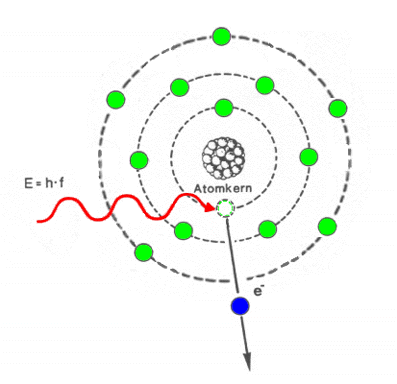
\includegraphics[width=.9\textwidth]{Figures/photoeffekt.png}
	    \caption{Schematische Darstellung der Wirkungsweise des Photoeffekts.\cite{bib:Photoeffekt}}\label{fig:Photoeffekt}
	  \end{minipage}\quad
	  \begin{minipage}{0.48\textwidth}
	    \centering
	    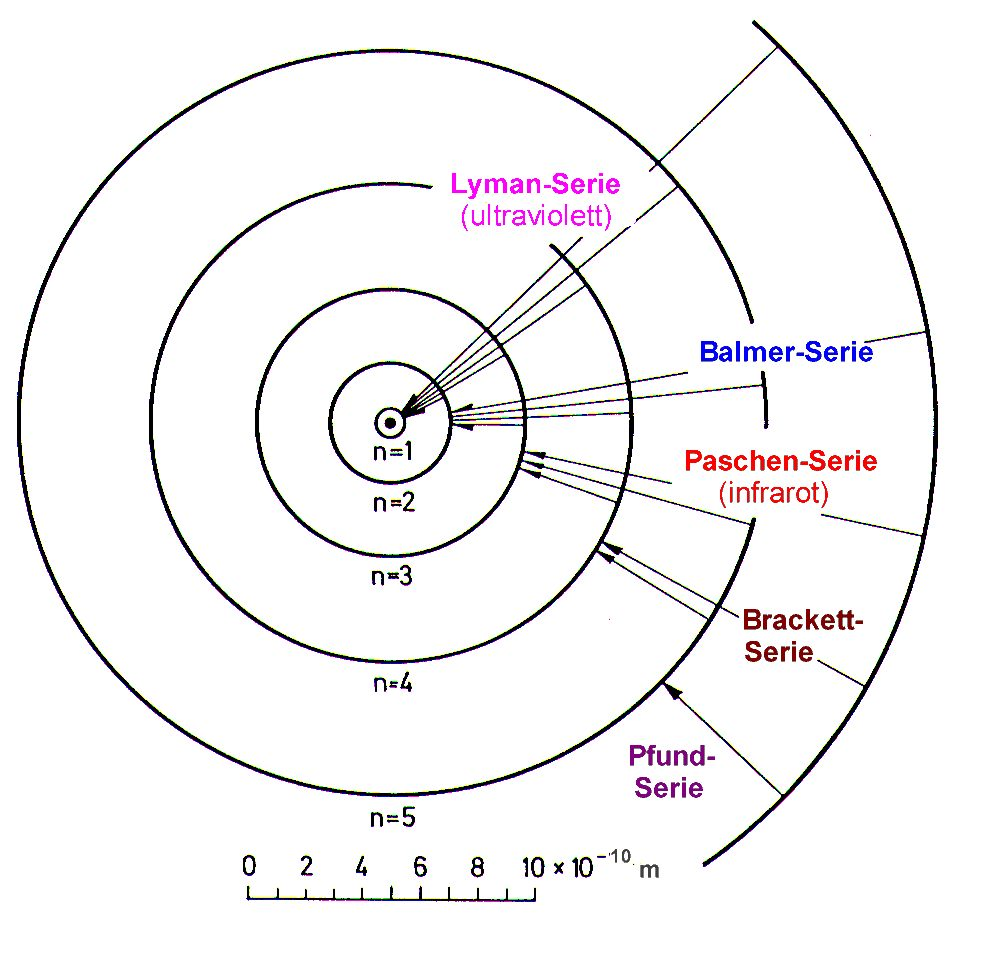
\includegraphics[width=.9\textwidth]{Figures/BohrschesAtommodellSerien.png}
	    \caption{Bohrsches Atommodell zusammen mit den Übergangsserien.\cite{bib:BohrschesAtommodellSerien}}\label{fig:BohrschesAtommodellSerien}
	  \end{minipage}
	\end{figure}
	
      \end{subsection}
      %%%%%%%%%%%%%%%%%%%%%%%%%%%%%%%%%%%%%%%%%%%%%%%%%%%%%%%%%%%%%%%%%%%%%%%%%%%%%%%%%%%%%%%%%%%%%%%%%%%%%%%%%%%%%%%%%%%%
      
      
      
      %%%%%%%%%%%%%%%%%%%%%%%%%%%%%%%%%%%%%%%%%%%%%%%%%%%%%%%%%%%%%%%%%%%%%%%%%%%%%%%%%%%%%%%%%%%%%%%%%%%%%%%%%%%%%%%%%%%%
      %%%%%%%%%%%%%%%%%%%%%%%%%%%%%%%%%%%%%%%%%%%%%%%%%%%%%%%%%%%%%%%%%%%%%%%%%%%%%%%%%%%%%%%%%%%%%%%%%%%%%%%%%%%%%%%%%%%%
      %%%%%%%%%%%%%%%%%%%%%%%%%%%%%%%%%%%%%%%%%%%%%%%%%%%%%%%%%%%%%%%%%%%%%%%%%%%%%%%%%%%%%%%%%%%%%%%%%%%%%%%%%%%%%%%%%%%%
      \begin{subsection}{Photozelle}
	\label{chp:TheoriePhotoelektrischesWirkungsquantumPhotozelle}
	In diesem Versuch wird der Photoeffekt u.A. dafür genutzt um Elektronen aus einer Metallplatte heraus zu lösen. Dabei trifft ein Laser mit einer ionisierenden Wellenlänge auf eine negativ geladene Metallplatte. Um ein Elektron aus der Oberfläche zu lösen muss die spezifische Austrittsarbeit des verwendeten Metalls erreicht werden. Aus der Austrittsarbeit ergibt sich mithilfe von \cref{eq:Grenzfrequenz} die sog. \textit{Grenzfrequenz}.
	\begin{equation}
	  \label{eq:Grenzfrequenz}
	  \nu_{0}=\frac{W_{A}}{h}
	\end{equation}
	Die ausgelösten Elektronen können anschließend in der Photozelle detektiert werden. Aufgebaut ist die Photozelle aus einem evakuierten Gehäuse in dem eine Metallplatte als Kathode angebracht ist. Auf der gegenüber liegenden Seite innerhalb des Gehäuses ist ein dünner Ringdraht als Anode angeschlossen. An Anode und Kathode kann nun eine Spannung angelegt werden um die ausgelösten Elektronen einem Potential auszusetzen. Wird nun Spannung erhöht, werden die Elektronen zur Anode hin beschleunigt und können als Strom mit einem Amperemeter gemessen werden. Wird die Spannung umgepolt, so werden die Elektronen zurück auf die Metallplatte beschleunigt und der Anodenstrom verringert sich. So kann man die kinetische Energie der ausgelösten Elektronen finden indem man die Grenzspannung bestimmt, bei der kein Anodenstrom mehr gemessen werden kann. Die maximale kinetische Energie ergibt sich dann aus der Differenz der Energie des Photons und der Austrittsarbeit mit \cref{eq:Ekin}.
	\begin{equation}
	  \label{eq:Ekin}
	  E_{kin}=eU_{0}=h\nu-W_{A}
	\end{equation}
	
	\begin{figure}[b]
	  \begin{center}
	    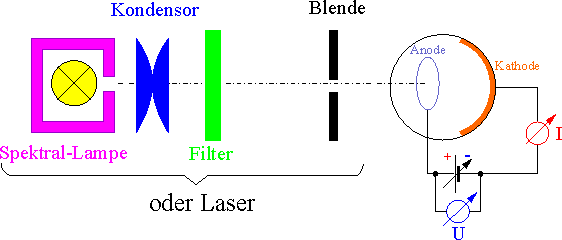
\includegraphics[width=.8\textwidth]{Figures/photozelle_mit_aufbau.png}
	    \caption{Schematischer Aufbau einer Photozelle.\cite{bib:PhotozelleAufbau}}\label{fig:PhotozelleAufbau}
	  \end{center}
	\end{figure}
	
	Um möglichst genaue Messwerte zu erhalten werden Anode und Kathode aus Materialien mit unterschiedlichen Ionisierungsenergien verwendet. Dadurch kann es vermieden werden, dass der Anodenstrom durch Elektronen verfälscht wird, die aus der Anode selbst gelöst wurden. Die Verbindung unterschiedlicher Materialien bringt allerdings den Nachteil mit sich, dass zwischen ihnen ein sog. \textit{Kontaktpotential} entsteht. Dieses Kontaktpotential entsteht, da sich die Potentiale (oder Fermi-Niveaus) beider Kontakte im Gleichgewicht befinden müssen. Daher kommt zu dieser Gleichung noch eine Korrektur für das Kontaktpotential zwischen den Materialien hinzu die in \cref{eq:KontaktpotentialKorrektur} gegeben ist.
	\begin{equation}
	  \label{eq:KontaktpotentialKorrektur}
	  W_{K}^{12}=\left|W_{A}^{1}-W_{A}^{2}\right|
	\end{equation}
	Daraus ergibt sich somit die Kontaktpotential korrigierte Formel für die kinetische Energie \cref{eq:EkinKontaktpotential}.
	\begin{equation}
	  \label{eq:EkinKontaktpotential}
	  E_{kin}=eU_{0}-W_{K}=h\nu-W_{A}-W_{K}
	\end{equation}
	
	\todo[inline]{Sind alle Formel richtig?}
	
      \end{subsection}
      %%%%%%%%%%%%%%%%%%%%%%%%%%%%%%%%%%%%%%%%%%%%%%%%%%%%%%%%%%%%%%%%%%%%%%%%%%%%%%%%%%%%%%%%%%%%%%%%%%%%%%%%%%%%%%%%%%%%
      
      
    \end{section}
    %%%%%%%%%%%%%%%%%%%%%%%%%%%%%%%%%%%%%%%%%%%%%%%%%%%%%%%%%%%%%%%%%%%%%%%%%%%%%%%%%%%%%%%
    
    
    
    %%%%%%%%%%%%%%%%%%%%%%%%%%%%%%%%%%%%%%%%%%%%%%%%%%%%%%%%%%%%%%%%%%%%%%%%%%%%%%%%%%%%%%%
    %%%%%%%%%%%%%%%%%%%%%%%%%%%%%%%%%%%%%%%%%%%%%%%%%%%%%%%%%%%%%%%%%%%%%%%%%%%%%%%%%%%%%%%
    %%%%%%%%%%%%%%%%%%%%%%%%%%%%%%%%%%%%%%%%%%%%%%%%%%%%%%%%%%%%%%%%%%%%%%%%%%%%%%%%%%%%%%%
    \begin{section}{Bohrsches Atommodell und Balmer-Serie}
      \label{chp:TheorieBohrBalmerSerie}
      
      
      
      %%%%%%%%%%%%%%%%%%%%%%%%%%%%%%%%%%%%%%%%%%%%%%%%%%%%%%%%%%%%%%%%%%%%%%%%%%%%%%%%%%%%%%%%%%%%%%%%%%%%%%%%%%%%%%%%%%%%
      %%%%%%%%%%%%%%%%%%%%%%%%%%%%%%%%%%%%%%%%%%%%%%%%%%%%%%%%%%%%%%%%%%%%%%%%%%%%%%%%%%%%%%%%%%%%%%%%%%%%%%%%%%%%%%%%%%%%
      %%%%%%%%%%%%%%%%%%%%%%%%%%%%%%%%%%%%%%%%%%%%%%%%%%%%%%%%%%%%%%%%%%%%%%%%%%%%%%%%%%%%%%%%%%%%%%%%%%%%%%%%%%%%%%%%%%%%
      \begin{subsection}{Aufbau des Borschen Atoms}
	\label{chp:TheorieBohrBalmerSerieAufbauAtomhuelle}
	Das Bohrsche Atommodell ist das wohl bekannteste Atommodell. Für sein Modell postulierte Bohr $1913$ die folgenden drei Postulate.
	\begin{enumerate}
	  \item Elektronen umkreisen den Atomkern auf festen Bahnen.
	  \item Das Elektron kann den Kern nur stabil und ohne Energieabstrahlung auf bestimmten, diskreten Bahnen mit festen Energien umkreisen.
	  \item Elektronen können ihre Energie nur durch Emission oder Absorption elektromagnetischer Strahlung ändern.
	\end{enumerate}
	Die Radien der diskreten Bahnen dieser Postulate sind mit \cref{eq:Bohrradius} und deren Energien mit \cref{eq:BohrradiusEnergien}.
	\newline
	\begin{minipage}{.48\textwidth}
	  \begin{equation}
	    \label{eq:Bohrradius}
	    r_{n}=\frac{n^{2}}{Z}a_{0}=\frac{n^{2}h^{2}\epsilon_{0}}{\pi\nu Ze^{2}}
	  \end{equation}
	\end{minipage}
	\begin{minipage}{.48\textwidth}
	  \begin{equation}
	    \label{eq:BohrradiusEnergien}
	    E_{n}=-R_{y}\frac{Z^{2}}{n^{2}}
	  \end{equation}
	\end{minipage}
	
	\todo[inline]{Hier muss noch was weiter gemacht werden. vielleicht etwas zu bahnwechseln ueber Absorption und Emission.}
	
      \end{subsection}
      %%%%%%%%%%%%%%%%%%%%%%%%%%%%%%%%%%%%%%%%%%%%%%%%%%%%%%%%%%%%%%%%%%%%%%%%%%%%%%%%%%%%%%%%%%%%%%%%%%%%%%%%%%%%%%%%%%%%
      
      
      
      %%%%%%%%%%%%%%%%%%%%%%%%%%%%%%%%%%%%%%%%%%%%%%%%%%%%%%%%%%%%%%%%%%%%%%%%%%%%%%%%%%%%%%%%%%%%%%%%%%%%%%%%%%%%%%%%%%%%
      %%%%%%%%%%%%%%%%%%%%%%%%%%%%%%%%%%%%%%%%%%%%%%%%%%%%%%%%%%%%%%%%%%%%%%%%%%%%%%%%%%%%%%%%%%%%%%%%%%%%%%%%%%%%%%%%%%%%
      %%%%%%%%%%%%%%%%%%%%%%%%%%%%%%%%%%%%%%%%%%%%%%%%%%%%%%%%%%%%%%%%%%%%%%%%%%%%%%%%%%%%%%%%%%%%%%%%%%%%%%%%%%%%%%%%%%%%
      \begin{subsection}{Spektroskopie}
	\label{chp:TheorieBohrBalmerSerieSpektroskopie}
	
	
	\begin{figure}[htbp]
	  \begin{center}
	    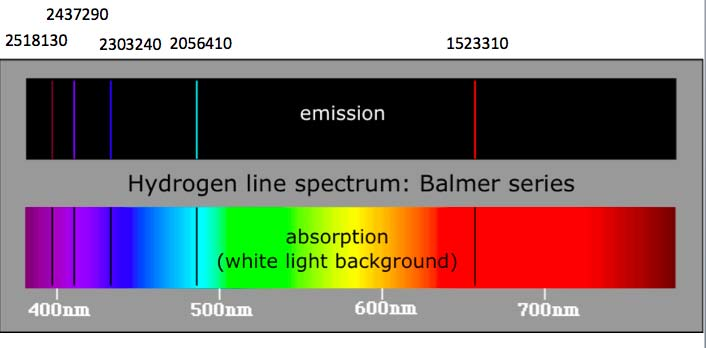
\includegraphics[width=.8\textwidth]{Figures/BalmerserieEmissionAbsorption.png}
	    \caption{Emissions- und Absorptionslinien der Balmer Übergänge im Wasserstoff Atom.\cite{bib:BalmerserieEmissionAbsorption}}\label{fig:BalmerserieEmissionAbsorption}
	  \end{center}
	\end{figure}
	
      \end{subsection}
      %%%%%%%%%%%%%%%%%%%%%%%%%%%%%%%%%%%%%%%%%%%%%%%%%%%%%%%%%%%%%%%%%%%%%%%%%%%%%%%%%%%%%%%%%%%%%%%%%%%%%%%%%%%%%%%%%%%%
      
      
    \end{section}
    %%%%%%%%%%%%%%%%%%%%%%%%%%%%%%%%%%%%%%%%%%%%%%%%%%%%%%%%%%%%%%%%%%%%%%%%%%%%%%%%%%%%%%%
    
  \end{chapter}
  %%%%%%%%%%%%%%%%%%%%%%%%%%%%%%%%%%%%%%%%%%%%%%%%%%%%%%%%%%
  
  
  
  %%%%%%%%%%%%%%%%%%%%%%%%%%%%%%%%%%%%%%%%%%%%%%%%%%%%%%%%%%
  %%%%%%%%%%%%%%%%%%%%%%%%%%%%%%%%%%%%%%%%%%%%%%%%%%%%%%%%%%
  %%%%%%%%%%%%%%%%%%%%%%%%%%%%%%%%%%%%%%%%%%%%%%%%%%%%%%%%%%
  \begin{chapter}{Versuchsaufbau und Durchführung}
    \label{chp:Aufbau}
    
    
    
    %%%%%%%%%%%%%%%%%%%%%%%%%%%%%%%%%%%%%%%%%%%%%%%%%%%%%%%%%%%%%%%%%%%%%%%%%%%%%%%%%%%%%%%
    %%%%%%%%%%%%%%%%%%%%%%%%%%%%%%%%%%%%%%%%%%%%%%%%%%%%%%%%%%%%%%%%%%%%%%%%%%%%%%%%%%%%%%%
    %%%%%%%%%%%%%%%%%%%%%%%%%%%%%%%%%%%%%%%%%%%%%%%%%%%%%%%%%%%%%%%%%%%%%%%%%%%%%%%%%%%%%%%
    \begin{section}{ERSTER TEIL}
      \label{chp:Aufbau:sec:ERSTERTEIL}
      
      
      
      %%%%%%%%%%%%%%%%%%%%%%%%%%%%%%%%%%%%%%%%%%%%%%%%%%%%%%%%%%%%%%%%%%%%%%%%%%%%%%%%%%%%%%%%%%%%%%%%%%%%%%%%%%%%%%%%%%%%
      %%%%%%%%%%%%%%%%%%%%%%%%%%%%%%%%%%%%%%%%%%%%%%%%%%%%%%%%%%%%%%%%%%%%%%%%%%%%%%%%%%%%%%%%%%%%%%%%%%%%%%%%%%%%%%%%%%%%
      %%%%%%%%%%%%%%%%%%%%%%%%%%%%%%%%%%%%%%%%%%%%%%%%%%%%%%%%%%%%%%%%%%%%%%%%%%%%%%%%%%%%%%%%%%%%%%%%%%%%%%%%%%%%%%%%%%%%
      \begin{subsection}{ERSTER UNTERTEIL}
	\label{chp:Aufbau:sec:ERSTERTEIL:subsec:UNTERTEIL}
       
       
       
      \end{subsection}
      %%%%%%%%%%%%%%%%%%%%%%%%%%%%%%%%%%%%%%%%%%%%%%%%%%%%%%%%%%%%%%%%%%%%%%%%%%%%%%%%%%%%%%%%%%%%%%%%%%%%%%%%%%%%%%%%%%%%
      
      
    \end{section}
    %%%%%%%%%%%%%%%%%%%%%%%%%%%%%%%%%%%%%%%%%%%%%%%%%%%%%%%%%%%%%%%%%%%%%%%%%%%%%%%%%%%%%%%
    
  \end{chapter}
  %%%%%%%%%%%%%%%%%%%%%%%%%%%%%%%%%%%%%%%%%%%%%%%%%%%%%%%%%%
  
  
  
  %%%%%%%%%%%%%%%%%%%%%%%%%%%%%%%%%%%%%%%%%%%%%%%%%%%%%%%%%%
  %%%%%%%%%%%%%%%%%%%%%%%%%%%%%%%%%%%%%%%%%%%%%%%%%%%%%%%%%%
  %%%%%%%%%%%%%%%%%%%%%%%%%%%%%%%%%%%%%%%%%%%%%%%%%%%%%%%%%%
  \begin{chapter}{Auswertung des Versuchs}
    \label{chp:Auswertung}
    
    
    
    %%%%%%%%%%%%%%%%%%%%%%%%%%%%%%%%%%%%%%%%%%%%%%%%%%%%%%%%%%%%%%%%%%%%%%%%%%%%%%%%%%%%%%%
    %%%%%%%%%%%%%%%%%%%%%%%%%%%%%%%%%%%%%%%%%%%%%%%%%%%%%%%%%%%%%%%%%%%%%%%%%%%%%%%%%%%%%%%
    %%%%%%%%%%%%%%%%%%%%%%%%%%%%%%%%%%%%%%%%%%%%%%%%%%%%%%%%%%%%%%%%%%%%%%%%%%%%%%%%%%%%%%%
    \begin{section}{ERSTER TEIL}
      \label{chp:Auswertung:sec:ERSTERTEIL}
      
      
      
      %%%%%%%%%%%%%%%%%%%%%%%%%%%%%%%%%%%%%%%%%%%%%%%%%%%%%%%%%%%%%%%%%%%%%%%%%%%%%%%%%%%%%%%%%%%%%%%%%%%%%%%%%%%%%%%%%%%%
      %%%%%%%%%%%%%%%%%%%%%%%%%%%%%%%%%%%%%%%%%%%%%%%%%%%%%%%%%%%%%%%%%%%%%%%%%%%%%%%%%%%%%%%%%%%%%%%%%%%%%%%%%%%%%%%%%%%%
      %%%%%%%%%%%%%%%%%%%%%%%%%%%%%%%%%%%%%%%%%%%%%%%%%%%%%%%%%%%%%%%%%%%%%%%%%%%%%%%%%%%%%%%%%%%%%%%%%%%%%%%%%%%%%%%%%%%%
      \begin{subsection}{ERSTER UNTERTEIL}
	\label{chp:Auswertung:sec:ERSTERTEIL:subsec:UNTERTEIL}
       
       
       
      \end{subsection}
      %%%%%%%%%%%%%%%%%%%%%%%%%%%%%%%%%%%%%%%%%%%%%%%%%%%%%%%%%%%%%%%%%%%%%%%%%%%%%%%%%%%%%%%%%%%%%%%%%%%%%%%%%%%%%%%%%%%%
      
      
    \end{section}
    %%%%%%%%%%%%%%%%%%%%%%%%%%%%%%%%%%%%%%%%%%%%%%%%%%%%%%%%%%%%%%%%%%%%%%%%%%%%%%%%%%%%%%%
    
  \end{chapter}
  %%%%%%%%%%%%%%%%%%%%%%%%%%%%%%%%%%%%%%%%%%%%%%%%%%%%%%%%%%
  
  
  
  %%%%%%%%%%%%%%%%%%%%%%%%%%%%%%%%%%%%%%%%%%%%%%%%%%%%%%%%%%
  %%%%%%%%%%%%%%%%%%%%%%%%%%%%%%%%%%%%%%%%%%%%%%%%%%%%%%%%%%
  %%%%%%%%%%%%%%%%%%%%%%%%%%%%%%%%%%%%%%%%%%%%%%%%%%%%%%%%%%
  \begin{chapter}{Fazit}
    \label{chp:Fazit}
    
    
    
    %%%%%%%%%%%%%%%%%%%%%%%%%%%%%%%%%%%%%%%%%%%%%%%%%%%%%%%%%%%%%%%%%%%%%%%%%%%%%%%%%%%%%%%
    %%%%%%%%%%%%%%%%%%%%%%%%%%%%%%%%%%%%%%%%%%%%%%%%%%%%%%%%%%%%%%%%%%%%%%%%%%%%%%%%%%%%%%%
    %%%%%%%%%%%%%%%%%%%%%%%%%%%%%%%%%%%%%%%%%%%%%%%%%%%%%%%%%%%%%%%%%%%%%%%%%%%%%%%%%%%%%%%
    \begin{section}{ERSTER TEIL}
      \label{chp:Fazit:sec:ERSTERTEIL}
      
      
      
      %%%%%%%%%%%%%%%%%%%%%%%%%%%%%%%%%%%%%%%%%%%%%%%%%%%%%%%%%%%%%%%%%%%%%%%%%%%%%%%%%%%%%%%%%%%%%%%%%%%%%%%%%%%%%%%%%%%%
      %%%%%%%%%%%%%%%%%%%%%%%%%%%%%%%%%%%%%%%%%%%%%%%%%%%%%%%%%%%%%%%%%%%%%%%%%%%%%%%%%%%%%%%%%%%%%%%%%%%%%%%%%%%%%%%%%%%%
      %%%%%%%%%%%%%%%%%%%%%%%%%%%%%%%%%%%%%%%%%%%%%%%%%%%%%%%%%%%%%%%%%%%%%%%%%%%%%%%%%%%%%%%%%%%%%%%%%%%%%%%%%%%%%%%%%%%%
      \begin{subsection}{ERSTER UNTERTEIL}
	\label{chp:Fazit:sec:ERSTERTEIL:subsec:UNTERTEIL}
       
       
       
      \end{subsection}
      %%%%%%%%%%%%%%%%%%%%%%%%%%%%%%%%%%%%%%%%%%%%%%%%%%%%%%%%%%%%%%%%%%%%%%%%%%%%%%%%%%%%%%%%%%%%%%%%%%%%%%%%%%%%%%%%%%%%
      
      
    \end{section}
    %%%%%%%%%%%%%%%%%%%%%%%%%%%%%%%%%%%%%%%%%%%%%%%%%%%%%%%%%%%%%%%%%%%%%%%%%%%%%%%%%%%%%%%
    
  \end{chapter}
  %%%%%%%%%%%%%%%%%%%%%%%%%%%%%%%%%%%%%%%%%%%%%%%%%%%%%%%%%%
  
  
  
  %%%%%%%%%%%%%%%%%%%%%%%%%%%%%%%%%%%%%%%%%%%%%%%%%%%%%%%%%%
  %%%%%%%%%%%%%%%%%%%%%%%%%%%%%%%%%%%%%%%%%%%%%%%%%%%%%%%%%%
  %%%%%%%%%%%%%%%%%%%%%%%%%%%%%%%%%%%%%%%%%%%%%%%%%%%%%%%%%%
  \begin{appendix}
    \label{Anhang}
    
    
    
    %%%%%%%%%%%%%%%%%%%%%%%%%%%%%%%%%%%%%%%%%%%%%%%%%%%%%%%%%%%%%%%%%%%%%%%%%%%%%%%%%%%%%%%
    %%%%%%%%%%%%%%%%%%%%%%%%%%%%%%%%%%%%%%%%%%%%%%%%%%%%%%%%%%%%%%%%%%%%%%%%%%%%%%%%%%%%%%%
    %%%%%%%%%%%%%%%%%%%%%%%%%%%%%%%%%%%%%%%%%%%%%%%%%%%%%%%%%%%%%%%%%%%%%%%%%%%%%%%%%%%%%%%
    \begin{chapter}{ERSTER TEIL}
      \label{Anhang:chp:ERSTERTEIL}
      
      
      
      %%%%%%%%%%%%%%%%%%%%%%%%%%%%%%%%%%%%%%%%%%%%%%%%%%%%%%%%%%%%%%%%%%%%%%%%%%%%%%%%%%%%%%%%%%%%%%%%%%%%%%%%%%%%%%%%%%%%
      %%%%%%%%%%%%%%%%%%%%%%%%%%%%%%%%%%%%%%%%%%%%%%%%%%%%%%%%%%%%%%%%%%%%%%%%%%%%%%%%%%%%%%%%%%%%%%%%%%%%%%%%%%%%%%%%%%%%
      %%%%%%%%%%%%%%%%%%%%%%%%%%%%%%%%%%%%%%%%%%%%%%%%%%%%%%%%%%%%%%%%%%%%%%%%%%%%%%%%%%%%%%%%%%%%%%%%%%%%%%%%%%%%%%%%%%%%
      \begin{section}{ERSTER UNTERTEIL}
	\label{Anhang:chp:ERSTERTEIL:sec:UNTERTEIL}
       
       
       
      \end{section}
      %%%%%%%%%%%%%%%%%%%%%%%%%%%%%%%%%%%%%%%%%%%%%%%%%%%%%%%%%%%%%%%%%%%%%%%%%%%%%%%%%%%%%%%%%%%%%%%%%%%%%%%%%%%%%%%%%%%%
      
      
    \end{chapter}
    %%%%%%%%%%%%%%%%%%%%%%%%%%%%%%%%%%%%%%%%%%%%%%%%%%%%%%%%%%%%%%%%%%%%%%%%%%%%%%%%%%%%%%%
    
  \end{appendix}
  %%%%%%%%%%%%%%%%%%%%%%%%%%%%%%%%%%%%%%%%%%%%%%%%%%%%%%%%%%
  
  
  
  %%%%%%%%%%%%%%%%%%%%%%%%%%%%%%%%%%%%%%%%%%%%%%%%%%%%%%%%%%
  %%%%%%%%%%%%%%%%%%%%%%%%%%%%%%%%%%%%%%%%%%%%%%%%%%%%%%%%%%
  %%%%%%%%%%%%%%%%%%%%%%%%%%%%%%%%%%%%%%%%%%%%%%%%%%%%%%%%%%
  \begin{thebibliography}{99}
    \scriptsize
    \bibitem{bib:PhotozelleAufbau}\url{http://www.leifiphysik.de/sites/default/files/medien/Kennlinie_einer_Fotozelle_Bild_2.gif}
    \bibitem{bib:Photoeffekt}\url{http://web-docs.gsi.de/~wolle/TELEKOLLEG/ATOM/IMAGES/photoeffekt1.gif}
    \bibitem{bib:BalmerserieEmissionAbsorption}\url{http://scienceblogs.de/primaklima/wp-content/blogs.dir/29/files/2012/06/i-86621a49589f7ddc22387aa065cef996-Balmerserie.jpg}
    \bibitem{bib:BohrschesAtommodellSerien}\url{http://www.systemdesign.ch/images/4/4e/BohrschesAtommodellSerien.jpg}
    
%     \cite{ALEPH:2005ab}
%     \bibitem{ALEPH:2005ab}
%     S.~Schael {\it et al.}  [ALEPH and DELPHI and L3 and OPAL and SLD and LEP Electroweak Working Group and SLD Electroweak Group and SLD Heavy Flavour Group Collaborations],
%     %``Precision electroweak measurements on the $Z$ resonance,''
%     Phys.\ Rept.\  {\bf 427} (2006) 257
%     [hep-ex/0509008];\\
%     %%CITATION = HEP-EX/0509008;%%
%     %868 citations counted in INSPIRE as of 16 Oct 2013
%     \texttt{http://lepewwg.web.cern.ch/LEPEWWG/plots/winter2012/}.
  \end{thebibliography}
  %%%%%%%%%%%%%%%%%%%%%%%%%%%%%%%%%%%%%%%%%%%%%%%%%%%%%%%%%%
  
\end{document}
%%%%%%%%%%%%%%%%%%%%%%%%%%%%%